\chapter{Technológiai háttér}
A feladat megoldásához szükséges ismerni a rendelkezésünkre álló technológiákat és azokat több szempontból megvizsgálni:
\begin{itemize}
    \item A legfontosabb természetesen az, hogy az adott technológia egyáltalán képes e biztosítani a követelményekben foglaltakat.
    \item A következő az implementáció könnyedsége és hatékonysága. Nem mindegy, hogy az adott technológiával csak megoldani tudjuk a problémát, az is fontos, hogy az valóban "arra legyen kitalálva" amire használni szeretnénk.
    \item A harmadik szempont bizonyos esetben fontosságban az implementációs könnyebbség elé is kerülhet: a költséghatékonyság. Már a dolgozatom írása során is előkerült egy jelentős különbség két szolgáltató között, melyről részletesebben az 5.1.-es fejezetben írok.
\end{itemize}
\section{Felhőszolgáltatások}
Napjainban egyre népszerűbb és költséghatékonyabb az úgynevezett \textit{Cloud Computing} lehetőségével élni. Ennek lényege, hogy nem szükséges saját magunknak a fizikai eszközöket (pl.: szervereket) beszerezni, hanem bérelhetünk egy szolgáltatótól számítási kapacitást. Többféle modell létezik, ezek közül a három legnépszerűbbet szeretném bemutatni:
\begin{itemize}
    \item Infrastructure as a Service (IaaS) - gyakorlatilag ez megfeleltethető egy távoli infrastruktúrának amiről máskülönben nekünk kellene gondoskodnunk. Ezek különböző komponensekből állhatnak, úgymint szerverek, tárterület, hálózat.
    \item Platform as a Service (PaaS) - hasonló a \textit{IaaS}-hoz, de itt több alkalmazásbeli réteget biztosítanak, például az operációs rendszert sem kell menedzselnünk többé, csupán az általunk futtatni kívánt alkalmazást és annak adatait.
    \item Software as a Service (SaaS) - gyakorlatilag a programok felhőben futó változata. Több olyan szoftver létezik aminek van úgynevezett \textit{self-hosted} (magunknak kiszolgált) változata és a kiadó által biztosított is.
\end{itemize}
\begin{figure}[ht]
\centering
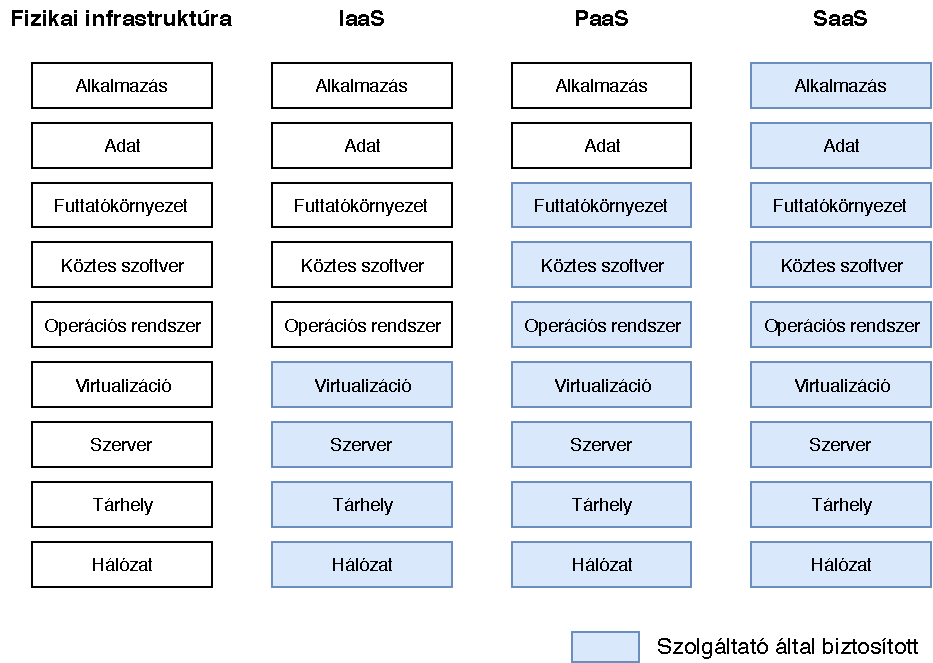
\includegraphics[width=150mm, keepaspectratio]{img/XaaS.pdf}
\caption{Különböző szolgáltatási modellek}
\end{figure}
\newpage
\vskip 0.1in
\subsection{Google Cloud Platform}
A Google 2008-ban indította útnak saját felhőszolgáltatását\footnote{\url{https://cloud.google.com/}}, ezzel komoly konkurenciát teremtve az Amazonnak aki akkor már két éve a piacon volt. Jelentős sikereket ért el, melyet legfőképp az infrastruktúra üzembiztonságának köszönhet, egy időben a marketing anyagokban is úgy fogalmaztak, hogy lehetőségünk van ugyanott futtatni alkalmazásainkat ahol a Google saját eszközei is megtalálhatóak.

Minden új felhasználónak lehetősége van igénybevenni 300 amerikai dollár kezdőegyenleget, mely szabadon felhasználható minden szolgáltatáshoz, illetve időnként promóciók keretében még többre is szert tehetünk (nemrég a GitLabbal szerződtek, így plusz 200 dollárhoz lehetett jutni). Nyújtanak továbbá oktatási támogatást is, azonban inkább projektekre és kutatásokra vonatkozik e kedvezmény, egy szakdolgozathoz én nem tudtam igénybevenni.

Szolgáltatási modellek terén megtalálható az \textit{Infrastructure as a Service}, ennek legfőbb terméke a \textit{Compute Engine}, ahol gyakorlatilag szervereket bérelhetünk általunk meghatározott operációs rendszerrel, és válaszhatunk többféle erőforrásmennyiség közül is. Érdekes megjegyezni, hogy válaszhatunk az adott feladathoz legjobban illő hardvert is, van például processzoroptimalizált és memóriaoptimalizált géptípus is. A \textit{Kubernetes Engine} a \textit{Platform as a Service} kategóriába sorolható és mint neve is mondja egy menedzselt Kubernetes klasztert ad számunkra, melyről később még szó fog esni. Ehhez kapcsolódik egy \textit{Software as a Service} szolgáltatás, mégpedig a \textit{Google Container Registry} ami egy konténerkép-tároló, melyről szintén szó fog esni, hogy pontosan mire szolgál. Természetesen több száz terméke létezik még a szolgáltatónak, de a dolgozatom megírása során közvetlenül ezzel a hárommal találkoztam.
\subsection{Amazon Web Services}
Az Amazon tulajdonában álló felhőszolgáltatás az ismertebbek közül a legrégebbi a piacon: az Amazon Web Services 2006 óta működik. Egyáltalán nem nevezhetjük olcsónak, azonban mivel az egyik legnagyobb tapasztalattal rendelkező cég, így sokan emiatt választják őket. 
\begin{figure}[ht]
\centering
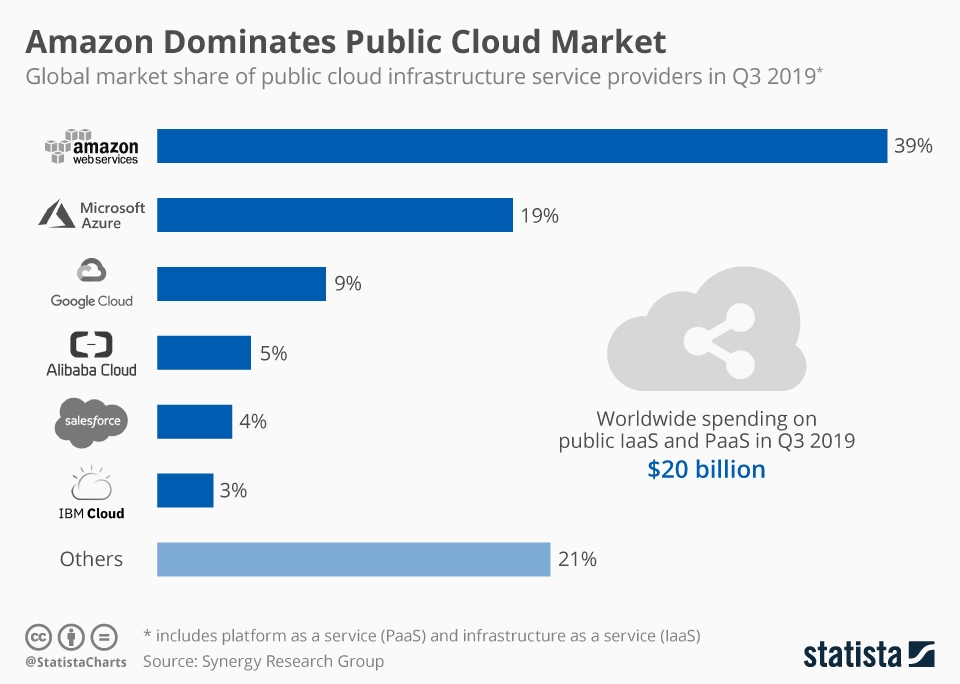
\includegraphics[width=150mm, keepaspectratio]{img/cloudproviders.jpg}
\caption{Felhőszolgáltatók piaci részesedése 2019-ben\cite{AWSshare}}
\end{figure}
\vskip 0.1in
Az új felhasználóknak úgynevezett \textit{free tier} (ingyenes szint) biztosított arra, hogy megismerje a terméket. Ezzel bár nem minden szolgáltatást lehet igénybevenni, de meg lehet ismerni mire képes a platform. Például ingyenesen lehet nagyon kis erőforráshasználatú szervert bérelni. Nyújtanak továbbá diákoknak havi 40 amerikai dollár támogatást, mely már több szolgáltatás használatára feljogosít. GitHub Student Developer Pack\footnote{\url{https://education.github.com/pack}} segítségével pedig további 110 dollárra tehetünk szert, mely már egész sok dolog kipróbálására elégséges.
\subsubsection{Elastic Compute Cloud (EC2)}
Az Amazon által nyújtott egyik legalapvetőbb \textit{Infrastructure as a Service} szolgáltatás, ahol rengeteg elődefiniált erőforráskombináció közül választhatjuk ki azt a géptípust amire nekünk szükségünk van. Természetesen ezen gépek az Amazon nagysebességű hálózatához csatlakoznak, és árkategóriától függően akár 10 Gbps sebességgel is tudnak a világhálón kommunikálni.
\subsubsection{Elastic Kubernetes Service (EKS)}
Az EKS egy menedzselt Kubernetes szolgáltatást biztosít mint \textit{Platform as a Service}. Fontos megjegyezni, hogy a worker számítógépekért (lásd: 3.4.1. fejezet) külön szükséges fizetni, hiszen azok gyakorlatilag előkonfigurált EC2 példányok. Az EKS egyébként sem mondható a legolcsóbb szolgáltatások közé, óránként 0.20 amerikai dollárt kell fizetnünk, és ez a workerek költségét nem is tartalmazza. Természetesen ez a havi 144\$ állandó összeg, tehát akár csak egy szolgáltatást futtatunk a klaszerben, akár ezret, ennyit fogunk fizetni a klaszter fenntartásáért.

A szolgáltatás nagymértékben integrálódik a lentebb felsorolt Amazon termékekkel, ezzel egy hatalmas előnyt állítva a saját kézzel összerakott Kubernetessel szemben.

\textit{Megjegyzés: az Amazonnak van egy saját - Kubernetes-szerű - szolgáltatása, az Elastic Container Service (ECS), mely lényegesen olcsóbb, nincs menedzsment költség, csak a workerekért kell fizetni.}
\subsubsection{Elastic Container Registry (ECR)}
Szintén egy későbbi fejezetben teszek említést a konténerekről, de röviden: alkalmazásainkat tárolhatjuk verziókezelt formában egy biztonságos, privát, és Kubernetes kompatibilis helyen. Előnye, hogy integrálódik az EKS-sel, illetve az Amazon jogosultságkezésével is (IAM).
\subsubsection{Virtual Private Cloud (VPC)}
Jogosan merül fel a kérdés, hogy például mi van akkor ha két kiszolgálót össze szeretnénk kötni hálózaton keresztül, de csak intraneten, helyi hálózaton. Hogy tehetjük meg ezt a felhőben? Sok egyéb mellett a VPC erre is alkalmas. Gyakorlatilag hálózatot építhetünk a felhőben.

A könnyebb áttekinthetőség érdekében tekintsük meg ezt az ábrát a hivatalos dokumentációból\cite{VPC}:
\newpage
\begin{figure}[!ht]
\centering
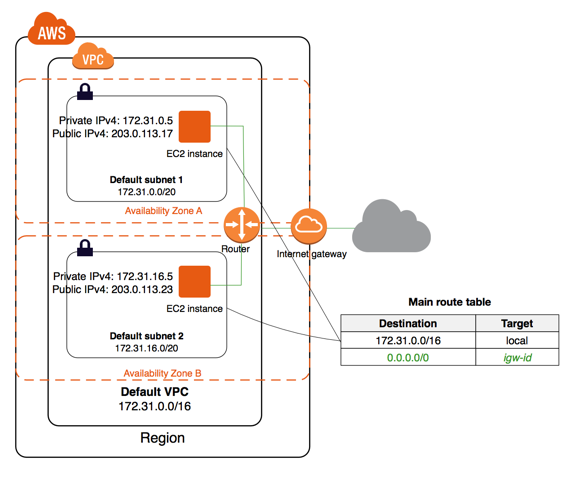
\includegraphics[width=150mm, keepaspectratio]{img/VPC.png}
\caption{A VPC működése}
\end{figure}
\vskip 0.1in
Az ábrán két kiszolgálót futtatunk (\textit{EC2 instance}), két külön elérhetőségi zónában (ezt azt jelenti, hogy bár egy régióban található a két adatközpont, azok izoláltak egymáshoz képest és egy alacsony késleltetésű kapcsolattal vannak összekötve). Mindkét kiszolgálónak van publikus és privát IP-címe is. Az elérhetőségi zónák között belső router irányítja a forgalmat, így az a publikus internet felé soha nem megy ki. A szándékosan külvilág felé/felől érkező csomagokat pedig az internet átjáró kezeli, mely szintén a routert használja.

Természetesen számos konfigurációs lehetőség van, például lehet ACL\footnote{Access Control List - kommunikáció/hozzáférés szabályozása}-eket beállítani. Az AWS alapértelmezetten konfigurál egy VPCt az EC2 példányoknak, és a szakdolgozatom kidolgozásához ez teljesen megfelelőnek bizonyult, így részletesebben nem térek ki a további lehetőségekre, azonban az alapvető működés megértését fontosnak gondolom.
\subsubsection{Elastic Load Balancing (ELB)}
Az Amazon terheléselosztója képes egy vagy több elérhetőségi zónán belül automatikusan elosztani az alkalmazások felé tartó forgalmat, legyen az EC2 példány, vagy egyéb szolgáltatások. Alapvetően kétféle terheléselosztót használhatunk, melyek mindegyike támogat olyan szolgáltatásokat mint a magas rendelkezésre állás, automatikus skálázódás illetve a beépített biztonsági funkciók:
\begin{itemize}
    \item Alkalmazásszintű terheléselosztó (\textit{Application Load Balancer}) - Leginkább HTTP és HTTPS forgalom elosztására tervezték, az OSI réteg\footnote{Open Systems Interconnection Reference Model, összesen hét szint} hetedik szintjén\footnote{Alkalmazásréteg} működik, és az Amazon VPC felé irányítja a kéréseket, azok tartalma alapján.
    \item Hálózati szintű terheléselosztó (\textit{Network Load Balancer}) - Leginkább TCP és UDP\footnote{User Datagram Protocol} forgalom elosztására tervezték, az OSI réteg negyedik szintjén\footnote{Szállítási réteg} működik, és az Amazon VPC felé irányítja a kéréseket, akár több milliót másodpercenként.
\end{itemize}
\subsubsection{Identity and Access Management (IAM)}
Egy hatalmas infrastruktúrához robosztus jogosultságkezelésre van szükség, és az Amazon IAM pontosan ezt valósítja meg. A szolgáltatás segítségével létrehozhatunk és menedzselhetünk AWS felhasználókat, csoportokat és jogosultságokat adhatunk nekik egy adott erőforrás elérésének engedélyezésére vagy megtagadására. Ha újrafelhasználni is szeretnénk egy adott engedélycsoportot akkor \textit{szerepbe} érdemes csoportosítani őket. A szerep engedélyek összessége és így egyszerűbben lehet adott személyhez, szolgáltatáshoz, vagy csoporthoz rendelni azt. Továbbá: ezeket a szerepeket meg lehet személyesíteni és fel lehet venni. Ezt azt jelenti, hogy nem kell mindenféleképp állandóan bírni egy adott jogosultsággal, csak amikor az ténylegesen indokolt. Például veszélyes lehet a napi munka során egy olyan jogkörrel bírni ami minden erőforrás törlésére jogosult, azonban néha előfordulhat hogy erre szükség van.
\section{Microservice architektúra}
Régen az emberek monolit alkalmazásokat írtak. Az ilyen típusú alkalmazások funkciói egyetlen kódbázisban, azaz egyetlen hatalmas programban valósulnak meg. Ez a fejlesztési fázis elején, kis projekteknél kényelmes, azonban hosszabbtávon nem kifizetődő.
\begin{figure}[!ht]
\centering
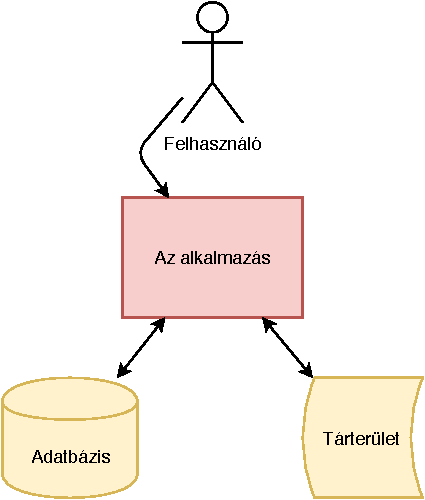
\includegraphics[width=60mm, keepaspectratio]{img/app_monolit.pdf}
\caption{A monolit alkalmazás felépítése}
\end{figure}
\vskip 0.1in
Mi is a probléma ezekkel a hatalmas alkalmazásokkal? Nagyobb terhelés mellett az egész szolgáltatás összeomolhat, még akkor is ha szorosan nem függnek egymástól az adott funkciók. Nehezen skálázható, csupán egy adott kiszolgálón futhat, nem lehet a részeit "szétszedni" és külön hardverre helyezni. A közös kódbázisból pedig a nehezebb fejleszthetőség problémája ered, hiszen mindenki ugyanazon forráskódot, továbbá elképzelhető, hogy az funkciók felelősei sincsenek teljesen pontosan meghatározva. (Például, hogy direkt vagy indirekt módon egy olyan osztálytól függ egy másik, melyről nem is gondolnánk).
\vskip 0.1in
A fenti leírásban már sugalltam, hogy mi a felsorolt problémákra a megoldás: találnunk kell egy módot, hogy valahogy izoláljuk alkalmazásunk egyes részeit, praktikusan funkcionalitás alapján.
\begin{figure}[!ht]
\centering
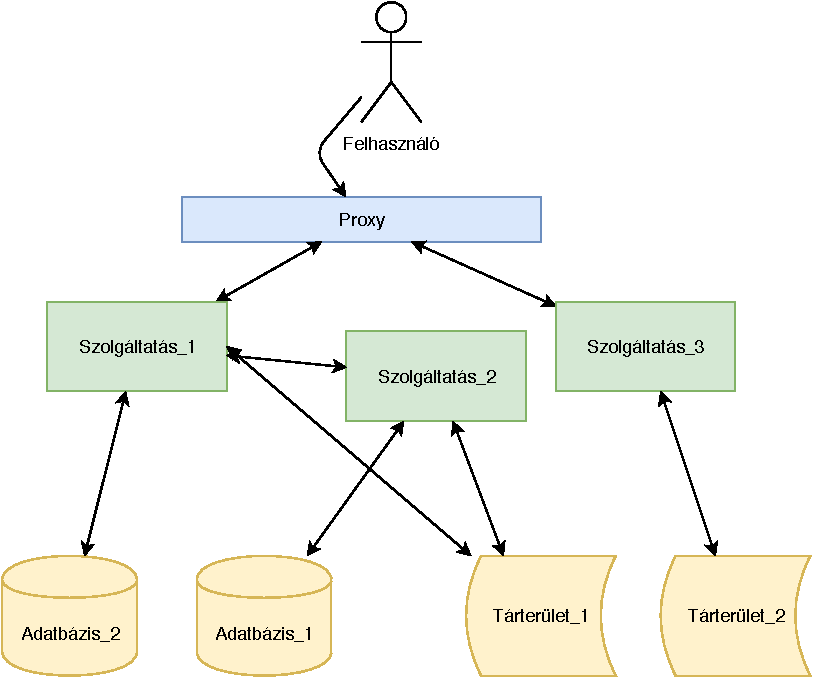
\includegraphics[width=125mm, keepaspectratio]{img/app_micro.pdf}
\caption{Egy egyszerűbb szolgáltatás, három mikroszolgáltatással megvalósítva}
\end{figure}
\vskip 0.1in
Az alkalmazásunk kódja is szeparált lett, könnyebb fejlesztőcsapatokat egy adott szolgáltatáshoz rendelni, továbbá a skálázhatóság is egyszerűbb, hiszen már akár több kiszolgálóra és elhelyezhetjük a különböző komponenseket. Ez utóbbit \textit{horizontális skálázás}nak nevezzük, míg mikor egy adott kiszolgálót bővítünk azt \textit{vertikális skálázásnak}.
\subsection{Stateful és stateless alkalmazások}
Tegyük fel, hogy hiába bontottuk szét alkalmazásunkat, az egyik mikroszolgáltatás olyan szintű terhelést kap, ami még egy dedikált kiszolgáló (tehát csak ezt az egy szolgáltatást futtatjuk) számára is kezelhetetlenül sok. Felmerülhet bennünk az ötlet, hogy indítsük el több példányban ezt a szolgáltatást és alkalmazzunk terheléselosztást a kettő között. Például egy fizetést megvalósító szolgáltatás ami egy \textit{Payment Gateway}\footnote{fizetési szolgáltatást biztosító "kapu"}-el kommunikál az ilymód skálázható, azonban ha mondjuk szeretnénk eltárolni azon felhasználók adatait akik fizettek, akkor ezen adatbázis nem. Miért? Mert a Payment Gateway API állapotmentes, nincs olyan amit tartósan tárolni kellene így mindegy melyik szolgáltatáshoz irányít minket a terheléselosztó. Egy adatbázisnak viszont pont a tárolás a lényege, így tulajdonképpen attól függene a visszaadott adathalmaz, hogy melyik példányhoz lettünk irányítva.

Előbbi szolgáltatást állapotmentesnek (\textit{statelessnek}, utóbbit pedig állapottól függőnek (\textit{statefulnak}) nevezünk. A stateful alkalmazások nehezen (vagy nem) skálázhatóak.
\section{Konténerizáció}
Régóta problémát jelentett, hogy egy adott alkalmazásnak számos függősége lehet, például hogy egy adott könyvtár/szoftver meglétére volt szükség hogy a programkód egyáltalán leforduljon. Ebből eredtek azok a problémák, hogy ami a fejlesztő gépén még futott az máshol már nem biztosan. Legnagyobb problémának viszont a függőségek úgynevezett ütközései bizonyoltak: tételezzük fel, hogy egyik alkalmazásunk \textbf{K könyvtár} 1.1-es verzióját szeretné használni, míg egy másik \textbf{K könyvtár} 2.0-s verzióját. Jobb esetben elfogadja az új a régit, de ez nem mindig ilyen egyszerű.

Erre a problémára is (és rengeteg, ennél fontosabbra is) megoldást találtak, mégpedig a \textit{virtualizáció}t. Ez a technológia lehetővé teszi egy fizikai kiszolgálón több logikai számítógép létrehozását a hardverelemek virtualizálásval. Ez azt jelenti, hogy a fizikai gépre (\textit{gazda}) telepítenünk kell egy \textit{hypervisor}t, mely az erőforrások elosztásáért és emulálásáért felelős. Ezek után a virtuális gépekre (\textit{vendég}) telepíteni kell operációs rendszert, és arra az alkalmazást. Hatékony technológia, és jelentősen megkönnyíti az erőforrások elosztását, költséghatékony megoldást teremtve.

Egy ideje azonban már a konténerizáció is jelen van, mely bizonyos tekintetben (természetesen több limitációval) hasonlít a virtualizációra és kevesebb erőforrást emészt fel a gazdagéptől. Az egyszerűbb megértés végett tekintsük meg ezt az ábrát:
\begin{figure}[ht]
\centering
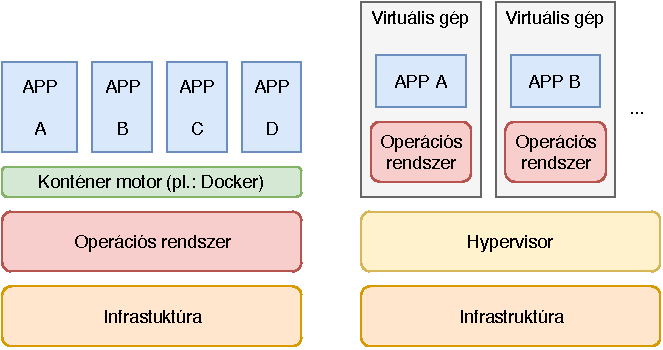
\includegraphics[width=125mm, keepaspectratio]{img/virtcont.pdf}
\caption{Konténerizáció és virtualizáció}
\end{figure}
\vskip 0.1in
Érdemes megfigyelni, hogy nincs többé szükségünk több operációs rendszer telepítésére, mely például egy Windows telepítés esetén súlyos "felesleges" erőforrást emésztene fel. Az ilymód futtatott alkalmazások a lehető legnagyobb mértékben izoláltan futnak, de egy közös operációs rendszeren, annak a szintjén szétválasztva. Több megoldás is létezik, például LXC, Jails vagy éppen a Docker.
\subsection{Docker}
A Docker 2013-ban látott napvilágot, azonban a kezdeti verziók meglehetősen instabilnak bizonyoltak. Ez az operációs rendszer szintű virtualizáció a Linux kernel számos képességét használja ki, mint például a névterek, a Netfilter vagy a cgroupok. A termék sikerességét bizonyítja, hogy a termék már MacOS-en és Windows rendszeren is használható.
A konténereket (amik gyakorlatilag a futtatható alkalmazások és függőségeik) \textit{kép}ekben tároljuk. Ha ilyen képet szeretnénk készíteni akkor úgynevezett \textit{Dockerfile}-t kell írnunk. A megadott utasítások alapján a Docker elvégzi a feladatot és utána a konténerkép segítségével konténerpéldányokat lehet indítnai.

Egy példa Dockerfile:
\begin{lstlisting}
FROM ubuntu:18.04      # az ubuntu konténerképből induluk ki, a 18.04es verzióból
COPY . /app            # a jelenlegi mappából a konténer /app mappájába másoljuk a fájlokat
RUN make /app          # a kép építése során végrehajtjuk a make /app parancsot
CMD python /app/app.py # a konténerkép futtatásakor az alábbi parancs fog végrehajtódni
\end{lstlisting}
\subsubsection{Registryk}
A Dockerfileban láttuk, hogy egy ubuntu képre hivatkozunk. De honnan van nekünk meg ez a kép? Nincsen. Egy Docker Hub nevű \textit{registry}ben tárolódik. A registryre úgy kell tekinteni mint egy konténerkép tároló. Ráadásul egyazon konténerből többféle verziót is közzétehetünk, ezt szolgálják a \textit{tag}ek melyet kettőspont után lehet írni (a fenti példában 18.04). Képet letölteni a \lstinline{pull}, feltölteni a helyi képek közül pedig a \lstinline{push} paranccsal lehet.

Létezek privát registryk is, hiszen nem mindenki szeretné az alkalamazását közzétenni az egész világ számára. Bár a Docker Hub is nyújt erre lehetőséget, ingyenesen csak egy repositorynk lehet, utána viszont fizetnünk kell, mégpedig nem keveset. Költséghatékonyabb megoldás például az \textit{Amazon Container Registryt (ECR)} használni, mely alapértelmezetten privát.
\section{Konténer orkesztráció}
Egy modern alkalmazás több száz mikroszolgáltatásból is állhat, melyek laza kötésű konténerekként jelennek meg. Konténer orkesztráció alatt ezen konténerek együttműködésének megszervezését jelentjük.\cite{ContOrch}

Több rendelkezésünkre álló technológia közül válaszhatunk, ilyen például az \textit{Apache Mesos}, \textit{Docker Swarm} és a \textit{Kubernetes}. Ezek mindegyike saját módszer alapján biztosítja a konténerek felügyeletetét, azok életciklusának kezelését, egészségüknek monitorozását, skálázását és frissítését.
\subsection{Kubernetes}
A Kubernetes 2014 nyarán jelent meg a Google gondozásában, és egy Dockerre épülő konténer orkesztrációs platformot valósít meg. Gyakran "k8s" néven is emlegetik.
\subsubsection{Alapfogalmak}
A Kubernetes alapvető működését objektumok határozzák meg, melyekből a fontosabbakat pár mondatban összefoglalom\cite{k8s}:
\begin{itemize}
    \item \textbf{Namespace} - A névterek egyfajta izolációs célt szolgálnak, gyakorlatilag egy virtuális klaszter a klaszterben.
    \item \textbf{Pod} - A Kubernetes legkisebb egysége. Konténerek összessége és az azokhoz tartozó alapvető konfigurációs beállítások mint például az igényelt erőforrások mennyisége.
    \item \textbf{Deployment} - A Deploymentek a Podok kezelésére szolgálnak. Megvalósíthatóak velük magas rendelkezésreállású szolgáltatások (több pod egyidejű futtatása), verziókezelés, skálázás.
    \item \textbf{Service} - Egy absztrakciós réteget von a Podok/Deployment hálózatkezelése felé. Megvalósít klaszteren belüli DNS bejegyzést és egy deployment alá tartozó podok felé érkező kommunikáció menedzselését.
    \item \textbf{Ingress} - A külvilágtól érkező kommunikációért felelős. Az adott Service HTTP és HTTPS útvonalait szolgálja ki, megadott szabályok alapján. Fontos, hogy az Ingress működéséhez egy úgynevezett Ingress Controllert kell telepíteni a klaszterbe, mely effektíve a forgalomirányítást végzi.
    \item \textbf{StatefulSet} - Az állapotfüggő szolgáltatások menedzselését hivatott elvégezni. Míg a deploymentnél teljesen lényegtelen például az indítási sorrend, addig egy stateful alkalmazásnál előfordulhat hogy ez igenis fontos.
    \item \textbf{ConfigMap} - Podok (és a bennük lévő konténerek) konfigurálására szolgál olymód, hogy azt nem közvetlen annak leíró fájlábab végezzük el, ezzel növelve az adott alkalmazás horozhatóságát. Fontos megjegyezni, hogy az érzékeny információk tárolására nem alkalmas, arra a \textit{Secret} objektum szolgál.
\end{itemize}
Ezeket az entitásokat úgynevezett \textit{.yaml} fájlban tudjuk leírni, ebből a negyedik fejezetben majd láthatunk párat.
\subsubsection{Magas rendelkezésre állás}
A Kubernetes segítségével szinte plusz befektetett energia nélkül tehetjük szolgáltatásunkat hibatűrővé. Egy Deployment létrehozásával és megfelelő konfigurálásával szinte azonnal elérhetjük célunkat. Frissítéskor úgynevezett \textit{Rolling Update} megy végbe: alapbeállítás szerint elindít egy podot, majd leállít egy régit. Ezt addig ismétli míg meghatározott számú pod nem lesz kész állapotban. Egy ilyen frissítésnél (és egyébként is) fontos megadni a Kubernetesnek, hogy hogyan tudja ellenőrizni hogy az alkalmazás elindult, illetve hogy nem hibásodott meg. Erre szolgál a \textit{ReadinessProbe} és a \textit{LivenessProbe}. Előbbi indításkor ellenőrzi mikor lesz kész a pod, utóbbi pedig már működés közben monitorozza azt. Ezek az ellenőrzések lehetnek egyszerű HTTP kérések, TCP ellenőrzés vagy egyéni alkalmazás futtatása konténeren belül.
\subsubsection{Terheléselosztás}
A Kubernetes a Service és az Ingress segítségével automatikusan elosztja az összetartozó podok közt a terhelést, így akár több állapotmentes alkalmazás tud ugyanazon feladat kisebb részeivel dolgozni.
\subsubsection{Skálázás}
A Kubernetes több szempont alapján és több módon teszi lehetővé a skálázást. Egyik legalapvetőbb módja a Deploymentben definiálni egy minimum és maximum podszám értéket, illetve hogy egy podnak milyen terhelést kell átlagosan kapnia hogy a skálázás végbemenjen.
\section{Verziókezelés}
Bár már többször említettem a verziókezelést dióhéjban, illetve annak fontosságát, a működését még nem írtam le. A lényeg alapvetően a változtatások követése, ezek verziózása és a lehetőség adott verzióra visszaállásra. Több megoldás létezik melyek implementációja eltér. Én most csak a Gitre fogok kitérni mivel az alkalmazás azt használja, de érdemes megemlíteni a \textit{Subversiont}, \textit{Mercurialt} és a \textit{Microsoft Team Foundation Servert} is.
\subsection{Git}
A Git szoftvert eredetileg Linus Torvalds fejlesztette ki a szintén általa írt Linux kernel forráskódjának kezelésére. Egyik legnagyobb újítása az volt, hogy nem kellett folyamatos kapcsolat egy központi szerverrel, hanem csak akkor kellett azt használni amikor szükség volt rá.

Megemlítek pár parancsot és azon keresztül adok egy alapvető képet a rendszer működéséről:
\begin{itemize}
    \item \textbf{commit} - Az elvégzett módosításokat egy új verzióba közzéteszi (de nem tölti fel a szerverre!)
    \item \textbf{push} - A repository lokális állapotát feltölti a szerverre.
    \item \textbf{clone} - Egy távoli szerveren lévő repositoryt tölt le a saját gépünkre.
    \item \textbf{pull} - A távoli szerveren lévő repository állapotát letölti és frissíti vele a lokálisat.
    \item \textbf{merge} - A paraméterül adott ágat az éppen aktuális ágba olvasztja.
    \item \textbf{rebase} - A paraméterül kapott ág commitjait alkalmazza az aktuális ágra.
    \item \textbf{revert} - Az adott commitra visszaállítja a repositoryt.
\end{itemize}
\subsection{GitHub}
A GitHub egy 2008-ban létrejött szolgáltatás, jelenleg a Microsoft tulajdonában. Megtalálható benne a Git összes "szerver" funkcionalitása és számos egyéb hozzáadott funkció is, például: hozzáférés-vezérlés, programhibák nyomonkövetése, wikicikkek írásának lehetősége, és rövid ideje már CI/CD funkcionalitást is találunk benne.

A szakdolgozatom szempontjából két fontos részt szeretnék kiemelni. Az egyik a pull requestek. Ezek több célt szolgálnak. Elsődleges funkcionalitása a főágra való beolvasztás áttekinthetőbbé tétele, illetve a közvetlenül főágra történő feltöltés tiltása. Publikus projekteknél például a közreműködés legszebb módja, ha letöltjük a kódot, egy külön ágon javítjuk a kódot, majd feltöltjük és pull requestet nyitunk. A másik fontos dolog, hogy a pull requestek arra is alkalmasak, hogy ezeken teszteket végezzünk, és csak akkor engedjük főágra a kódot ha ez sikeres volt. Többek között a fenti két szabály is megtalálható az úgynevezett \textit{Branch Protection Rules} között, mely a GitHub online felületén konfigurálható.
\section{CI/CD}
Ahogyan azt az 1.1.1.-es fejezetben kifejtettem, a \textit{Continuous Integration} és \textit{Continuous Deployment} rendkívül hasznos dolog, és értékes mérnökórákat lehet megtakarítani egy jól kidolgozott folyamat során, ugyanis se a projektek közti koordinációra, se az esetleges (CI hiányából fakadó) alkalmazáshibákra nem kell időt fordítani.

Jelenleg több szolgáltató is van aki különféle megoldásokat kínál. Talán az egyik legnépszerűbb a GitHubhoz használható \textit{Travis CI}, de már maguk a kódot tároló szolgáltatók is előálltak megoldásokkal. A \textit{GitLabon} hosszú ideje létezik erre megoldás, a GitHub pedig az utóbbi fél év óta szintén kínál hasonló szolgáltatást\cite{GHAction}. Azonban én a szakdolgozatom során egy - mondhatni - ipari sztendertet fogok használni, a Jenkinst.
\subsection{Jenkins}
A szoftver 2005-ben került először piacra, akkor még \textit{Hudson} néven, a Sun Microsystemstől. 2011-ben nevezték át Jenkinsre (egészen pontosan leágaztatták). Sikerét konfigurálhatóságának és testreszabhatóságának köszönheti. Több száz bővítmény érhető el hozzá, és a folyamatokat Groovy nyelven is leírhatjuk.

Az alkalmazás alapvetően egy mesterből áll, és ezekhez lehet dolgozókat csatolni a teljesítmény növelése céljából. A mestert szintén be lehet állítani, hogy részt vegyen a munkában is.
\section{Monitorozás}
Egy szolgáltatásnak sem szabadna léteznie megfelelő monitorozás nélkül. Sajnos eddigi tapasztalataim alapján ezt sokan nem így látják és nem fektetnek ebbe energiát. Monitorozás alatt azt értem, hogy a szolgáltatást és/vagy az azt futtató infrastruktúrát valamilyen módon megfigyeljük (természetesen célszoftverekkel) és rendellenesség esetén súlyosságtól függően tájékoztatjuk az illetékes személyt a megfelelő csatornák igénybevételével.

Több szoftver is elérhető, régen a Zabbix volt a sztendert, de mára idejétmúltnak mondhatjuk. Ez a megoldás agentek telepítését követelte meg a monitorozni kívánt entitásra, és a metrikák úgynevezett \textit{push} módon érkeztek meg a Zabbix szerverhez ahol aztán azok feldolgozásra kerültek. Manapság inkább a Prometheus által kínált megoldást használják.
\subsection{Prometheus}
2014-ben kezdődött el a szoftver fejlesztése, Go programozási nyelvben. Ez azért érdekes mert minden komponens egy-egy binárisnak felel meg, nem szükséges telepítés. A Prometheus újdonságát az adja, hogy \textit{pull} módszerrel szerzi be a metrikákat: úgynevezett \textit{exporter}eket lehet telepíteni a monitorozandó entitásra \textit{vagy} egyéb helyre is. Ez a Go bináris egy apró webszerver segítségével teszi közzé az adatokat, amit a Prometheus konfigurálható időközönként beolvas és értelmez. Ezt nevezik \textit{scrape} műveletnek.

Természetesen az adatok gyűjtése még nem minősül monitorozásnak, arról riasztást is kell kapnia az érintetteknek. A Prometheushoz külön binárisban letölthető az \textit{AlertManager}, mely csoportosítja, deduplikálja a riasztásokat majd elküldi azokat, illetve figyeli ha egy aktív riasztás megoldódik. Természetesen karbantartási ablakokat is meg lehet határozni.
\subsection{Grafana}
Egy beérkező riasztás leírása nem minden esetben elég beszédes ahhoz, hogy meg tudjuk határozni pontosan hol van a hiba a rendszerben. Szükséges valamilyen vizualizációs eszköz is, erre pedig a tökéletes megoldás a Grafana nevű eszköz.
\begin{figure}[ht]
\centering
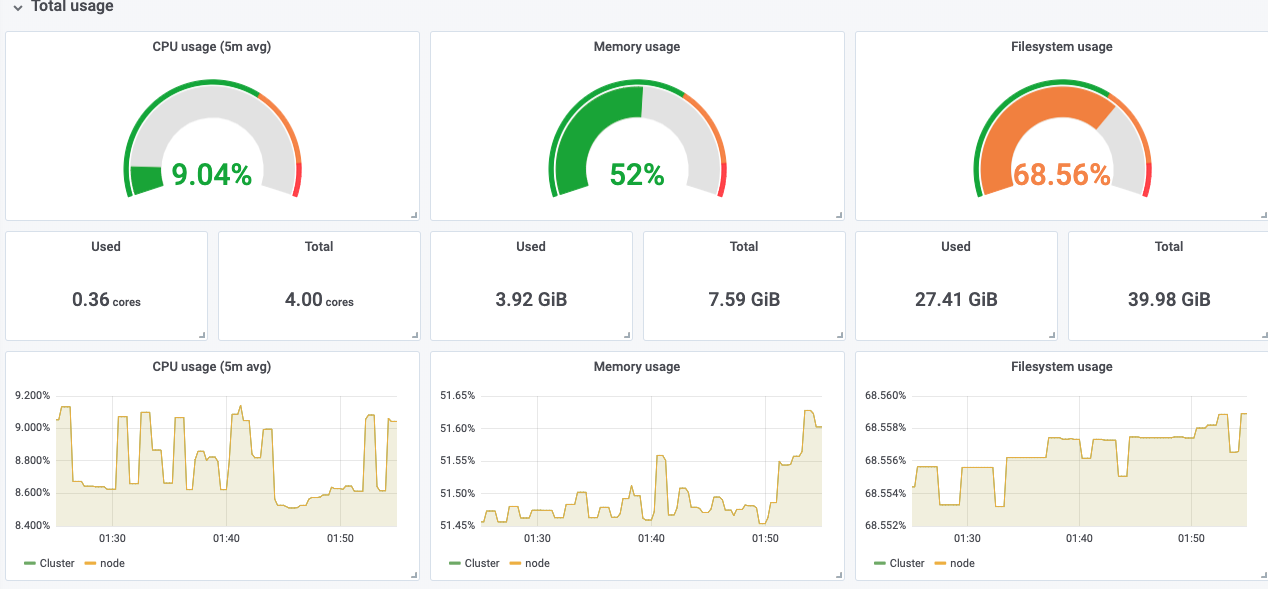
\includegraphics[width=150mm, keepaspectratio]{img/grafanaui.png}
\caption{A Grafana felhasználói felülete}
\end{figure}
\vskip 0.1in
A felületen különböző nézetek (\textit{dashboardok}) közül lehet választani, és ezeken \textit{Panel}ek jelenítik meg az adatot. Az adatok lekérdezésének a nyelve Prometheus adatforrás esetén \textit{PromQL}. Bár a Grafana felületén is lehetőség van riasztások létrehozására, személyes tapasztalatom alapján ez messze nem éri el az AlertManager (vagy hasonló technológiák) szintjét.